\chapter{Síntese assimétrica}\label{ch:b3:asymmetric-synthesis}

A L-DOPA, o fármaco que alivia os sintomas da doença de Parkinson, foi, na
década de 1970, o primeiro composto produzido industrialmente por \omterm{def:b3:asymmetric-synthesis:asymmetric-catalysis}{catálise assimétrica}: alguns
gramas de um complexo quiral de ródio, dissolvidos com um precursor plano e aquiral
sob hidrogênio, deram um produto no qual um enantiômero superava de longe o
outro. Os dois enantiômeros de um fármaco podem diferir completamente em seus efeitos,
porque os receptores e as \omterm{def:b3:complex-kinetics:enzyme}{enzimas} que eles encontram são eles próprios quirais. Este
capítulo mede a pureza enantiomérica, explica como um ambiente quiral escolhe
entre dois caminhos especulares e percorre as estratégias (\omterm{def:b3:asymmetric-synthesis:chiral-pool}{reservatório quiral},
auxiliares, resoluções, catalisadores metálicos e orgânicos) que produzem enantiômeros
puros.

\begin{recall}
O volume do 1.º ano definiu a quiralidade, os enantiômeros, os diastereoisômeros, as misturas
racêmicas, o poder rotatório específico, as regras CIP e as reações estereosseletivas e
estereoespecíficas; o volume do 2.º ano, a hidrogenação catalítica, a
epoxidação, a di-hidroxilação, as iminas, as enaminas, os enolatos, a reação aldólica,
a anelação de Robinson e a cromatografia. O \cref{ch:b3:rate-theories} deu a
\omterm{thm:b3:rate-theories:eyring}{equação de Eyring}, o \cref{ch:b3:homogeneous-catalysis}, o ciclo de Wilkinson, e o
\cref{ch:b3:point-groups}, o eixo $C_2$.
\end{recall}

\begin{omfigure}
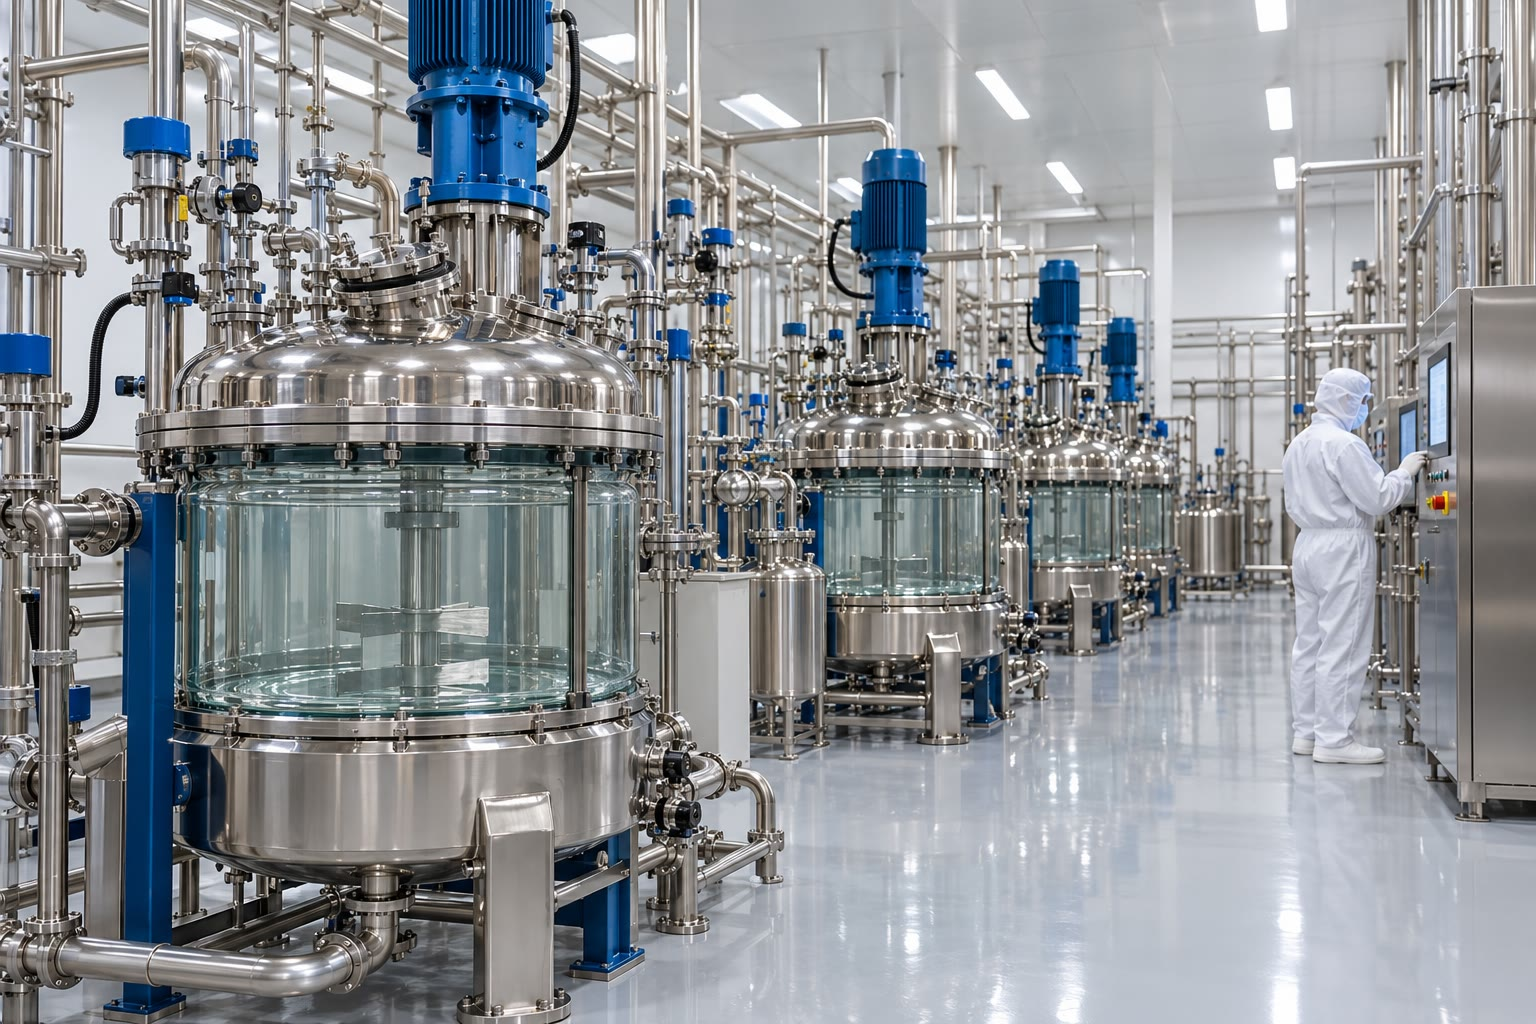
\includegraphics[width=0.58\linewidth]{images/book4/ai/b3-28-api-plant.jpg}

{\small Um salão de reatores revestidos de vidro em uma fábrica de princípios ativos
farmacêuticos. Muitos de seus produtos são enantiômeros puros, obtidos
por catálise ou por resolução e controlados por cromatografia quiral.}
\end{omfigure}

\section{Medir a pureza enantiomérica}

\begin{definition}[Excesso enantiomérico]\label{def:b3:asymmetric-synthesis:ee}
Para uma mistura de enantiômeros em quantidades $n_R \ge n_S$, o \emph{excesso
enantiomérico}\index{excesso enantiomerico@excesso enantiomérico} é $\mathrm{ee} = (n_R - n_S)/(n_R + n_S)$ e a \emph{razão enantiomérica}%
\index{razao enantiomerica@razão enantiomérica} é $\mathrm{er} = n_R/n_S$; para os diastereoisômeros, o
\emph{excesso diastereoisomérico}\index{excesso diastereoisomerico@excesso diastereoisomérico} de é definido da
mesma maneira. A \emph{pureza óptica}\index{pureza optica@pureza óptica} é a razão entre o
poder rotatório específico de uma amostra e o do enantiômero puro.
\end{definition}

\begin{proposition}[ee e er]\label{prop:b3:asymmetric-synthesis:ee-er}
$\mathrm{ee} = (\mathrm{er} - 1)/(\mathrm{er} + 1)$ e $\mathrm{er} = (1 + \mathrm{ee})/(1 - \mathrm{ee})$.
\end{proposition}

\begin{proof}
Divida o numerador e o denominador de $(n_R - n_S)/(n_R + n_S)$ por $n_S$; resolvendo para er, obtém-se a
segunda forma.
\end{proof}

Um ee de 90\,\% corresponde a um er de 95\,:\,5, um ee de 98\,\% a um er de 99\,:\,1. A \omterm{def:b3:asymmetric-synthesis:ee}{pureza óptica}
só é igual ao ee se o poder rotatório for proporcional à composição; as impurezas, o
solvente, os efeitos de concentração e os pequenos poderes rotatórios de muitos compostos a tornam
pouco confiável, e o ee é medido separando os enantiômeros.

\begin{method}[ee a partir de um cromatograma quiral]\label{met:b3:asymmetric-synthesis:ee-chromatogram}
\begin{enumerate}
  \item Injete primeiro o racemato, para identificar os dois picos e verificar sua
        separação (resolução até a linha de base) e suas áreas iguais.
  \item Injete a amostra e integre os dois picos.
  \item Os enantiômeros têm a mesma resposta em um detector aquiral, de modo que
        $\mathrm{ee} = (A_1 - A_2)/(A_1 + A_2)$; atribua os picos com um padrão enantiopuro.
\end{enumerate}
\end{method}

\begin{omfigure}
\begin{tikzpicture}
\begin{axis}[name=a, width=0.48\linewidth, height=5.4cm, xmin=0, xmax=20, ymin=0, ymax=1.0,
  axis lines=left, xlabel={$\Delta\Delta G^\ddagger$ / \unit{kJ.mol^{-1}}}, ylabel={ee},
  tick label style={font=\scriptsize}, label style={font=\small}]
\addplot[omDef, thick] table[x=ddg, y=eeA] {figdata/out/bachelor-3-er-ddg.dat};
\addplot[omMeth, thick] table[x=ddg, y=eeB] {figdata/out/bachelor-3-er-ddg.dat};
\addplot[omThm, thick] table[x=ddg, y=eeC] {figdata/out/bachelor-3-er-ddg.dat};
\node[font=\scriptsize, omDef, anchor=west] at (axis cs:10,0.55) {\qty{-78}{\celsius}};
\node[font=\scriptsize, omMeth, anchor=west] at (axis cs:10,0.43) {\qty{0}{\celsius}};
\node[font=\scriptsize, omThm, anchor=west] at (axis cs:10,0.31) {\qty{25}{\celsius} (mais baixa)};
\end{axis}
\begin{axis}[at={(a.east)}, anchor=west, xshift=1.4cm, width=0.48\linewidth, height=5.4cm,
  xmin=7.5, xmax=9.5, ymin=0, axis lines=left, ytick=\empty,
  xlabel={tempo de retenção / min}, ylabel={sinal do detector},
  tick label style={font=\scriptsize}, label style={font=\small}]
\addplot[black, thick] table[x=t, y=y] {figdata/out/bachelor-3-er-ddg-b.dat};
\node[font=\scriptsize, anchor=south west] at (axis cs:8.3,250) {(\textit{R}): 97.5};
\node[font=\scriptsize, anchor=south] at (axis cs:9.1,20) {(\textit{S}): 2.5};
\end{axis}
\end{tikzpicture}

{\small À esquerda: \omterm{def:b3:asymmetric-synthesis:ee}{excesso enantiomérico} em função da diferença de \omterm{def:b3:rate-theories:activation}{energia de Gibbs de
ativação} dos dois caminhos concorrentes, a três temperaturas: o mesmo
$\Delta\Delta G^\ddagger$ dá um ee mais alto a baixa temperatura. À direita: um cromatograma de HPLC quiral,
áreas de pico 97.5 e 2.5 (modelo): ee 95\,\%.}
\end{omfigure}

A RMN só distingue os enantiômeros em um ambiente quiral: um agente de solvatação
quiral forma complexos diastereoisoméricos de vida curta cujos sinais diferem, e um
álcool ou uma amina quiral convertido em seus dois ésteres diastereoisoméricos com
o ácido de Mosher revela a configuração pelo padrão das diferenças de deslocamento.

\begin{method}[Configuração a partir dos ésteres de Mosher, em linhas gerais]\label{met:b3:asymmetric-synthesis:mosher}
\begin{enumerate}
  \item Prepare os dois ésteres de MTPA, (\textit{R}) e (\textit{S}), do álcool.
  \item Registre seus espectros de prótons e calcule $\Delta\delta = \delta_S - \delta_R$ para os prótons de cada
        lado do carbono carbinólico.
  \item Na conformação preferida, o anel fenila do ácido blinda um dos lados:
        os prótons com $\Delta\delta > 0$ ficam de um lado, os com $\Delta\delta < 0$ do outro, o que
        situa os dois substituintes e dá a configuração.
\end{enumerate}
\end{method}

\section{Topicidade e adições estereosseletivas}

\begin{definition}[Reações estereosseletivas]\label{def:b3:asymmetric-synthesis:selective}
Uma \emph{reação enantiosseletiva}\index{reacao enantiosseletiva@reação enantiosseletiva} forma um
enantiômero de um produto em excesso em relação ao outro; uma \emph{reação
diastereosseletiva}\index{reacao diastereosseletiva@reação diastereosseletiva} forma um diastereoisômero em excesso.
\end{definition}

\begin{definition}[Topicidade]\label{def:b3:asymmetric-synthesis:topicity}
Dois grupos de uma molécula são \emph{homotópicos}\index{homotopicos@homotópicos} quando trocados por
uma rotação da molécula (substituir um ou outro dá o mesmo composto),
\emph{enantiotópicos}\index{enantiotopicos@enantiotópicos} quando trocados apenas por uma reflexão
(substituir um ou outro dá enantiômeros), e
\emph{diastereotópicos}\index{diastereotopicos@diastereotópicos} quando nenhuma \omterm{def:b3:point-groups:operation}{operação de simetria} os troca
(substituir um ou outro dá diastereoisômeros).
\end{definition}

Os dois hidrogênios de um grupo $\ce{CH2}$ vizinho a um estereocentro são \omterm{def:b3:asymmetric-synthesis:topicity}{diastereotópicos}: eles
têm deslocamentos químicos diferentes e se acoplam entre si, e é por isso que um grupo desse tipo
aparece muitas vezes como dois sinais em RMN.

\begin{definition}[Faces pró-quirais]\label{def:b3:asymmetric-synthesis:faces}
Um carbono trigonal com três substituintes diferentes é \emph{pró-quiral}\index{pro-quiral@pró-quiral}:
a adição de um quarto grupo, diferente, cria um estereocentro. Sua face vista com
os três substituintes em prioridade CIP decrescente no sentido horário é a
\emph{face Re}\index{face Re}; no sentido anti-horário, a \emph{face Si}\index{face Si}.
\end{definition}

\begin{omfigure}
\begin{tikzpicture}[font=\small, >=Stealth]
  \coordinate (c) at (0,0);
  \draw[thick, double, double distance=1.6pt] (c) -- (90:1.1) node[above] {O (1)};
  \draw[thick] (c) -- (210:1.1) node[below left] {$\ce{C6H5}$ (2)};
  \draw[thick] (c) -- (330:1.1) node[below right] {$\ce{CH3}$ (3)};
  \fill (c) circle (1.6pt);
  \draw[->, thick, omThm] (70:0.6) arc[start angle=70, end angle=200, radius=0.6];
  \node[font=\scriptsize, omThm, align=center] at (-1.9,0.75) {1 $\to$ 2 $\to$ 3\\ anti-horário:\\ face \textit{Si}};
  \node[font=\scriptsize, align=left, anchor=west] at (2.6,0.4) {face voltada para o leitor: \textit{Si}\\ face atrás da página: \textit{Re}};
  \node[font=\scriptsize, align=left, anchor=west] at (2.6,-0.5) {hidreto adicionado pela face \textit{Re}\\ dá o (\textit{S})-1-feniletanol};
\end{tikzpicture}

{\small As faces da acetofenona. Vistos de frente, os substituintes do
carbono carbonílico em ordem CIP (O, fenila, metila) giram no sentido anti-horário: a face
da frente é \textit{Si}, a de trás, \textit{Re}.}
\end{omfigure}

\begin{method}[Atribuir as faces Re e Si]\label{met:b3:asymmetric-synthesis:re-si}
\begin{enumerate}
  \item Ordene os três substituintes do átomo trigonal pelas regras CIP (uma
        ligação dupla conta seu parceiro duas vezes).
  \item Olhe a face de interesse, com o plano trigonal no plano da página.
  \item Sentido horário 1 $\to$ 2 $\to$ 3: \textit{Re}; anti-horário: \textit{Si}.
  \item Para nomear o produto, acrescente o novo grupo voltado para o observador e aplique as
        regras CIP ao novo estereocentro; o ataque pela \omterm{def:b3:asymmetric-synthesis:faces}{face Re} nem sempre dá \textit{R}.
\end{enumerate}
\end{method}

\begin{definition}[Modelo de Felkin--Anh e controle por quelação]\label{def:b3:asymmetric-synthesis:felkin}
O \emph{modelo de Felkin--Anh}\index{modelo de Felkin--Anh} prevê o diastereoisômero
majoritário de uma adição nucleofílica a um grupo carbonila vizinho a um
estereocentro: o maior grupo desse centro fica perpendicular ao
plano da carbonila, e o nucleófilo se aproxima em anti a ele, passando pelo menor
grupo, ao longo da trajetória de Bürgi--Dunitz. Sob \emph{controle por
quelação}\index{controle por quelacao@controle por quelação}, um íon metálico ligado ao mesmo tempo ao oxigênio carbonílico
e a um grupo doador do estereocentro trava a conformação, e o
nucleófilo se adiciona à face menos impedida do anel quelato.
\end{definition}

\begin{proposition}[Seletividade de Felkin--Anh]\label{prop:b3:asymmetric-synthesis:felkin}
Para um aldeído ou uma cetona $\alpha$-quiral sem grupo quelante, o produto
majoritário é o previsto pelo \omterm{def:b3:asymmetric-synthesis:felkin}{modelo de Felkin--Anh} (um modelo empírico,
apoiado por cálculos). \admitted
\end{proposition}

\begin{omfigure}
\begin{tikzpicture}[font=\small, >=Stealth]
  \foreach \a/\lab in {90/L, 330/M, 210/S} {
    \draw[line width=0.8pt] (\a:0.55) -- (\a:1.1) node[pos=1.3] {\lab};
  }
  \fill[white] (0,0) circle (0.55);
  \draw[line width=0.8pt] (0,0) circle (0.55);
  \draw[line width=0.8pt, double, double distance=1.4pt] (0,0) -- (0:1.1) node[right] {O};
  \draw[line width=0.8pt] (0,0) -- (180:1.1) node[left] {R};
  \draw[->, very thick, omThm] (250:2.2) -- (250:0.25);
  \node[omThm, anchor=north] at (250:2.25) {Nu$^-$};
  \node[font=\scriptsize, align=left, anchor=west] at (1.7,-1.0) {Nu$^-$ entra em anti a L,\\ passando por S, a cerca de 107°\\ da ligação C=O};
\end{tikzpicture}

{\small \omterm{def:b3:asymmetric-synthesis:felkin}{Modelo de Felkin--Anh}, visto ao longo da ligação do carbono carbonílico (à frente,
ligações com O e R) ao estereocentro (círculo atrás, grupos L, M e S). O
grupo grande fica perpendicular ao plano da carbonila; o nucleófilo vem do
lado oposto, perto do grupo pequeno e longe do oxigênio.}
\end{omfigure}

\section{Estratégias}

\begin{definition}[Reservatório quiral]\label{def:b3:asymmetric-synthesis:chiral-pool}
O \emph{reservatório quiral}\index{reservatorio quiral@reservatório quiral} é o conjunto dos compostos naturais
baratos e enantiopuros (aminoácidos, açúcares, terpenos, hidroxiácidos) usados como
materiais de partida, cujos estereocentros são levados até o alvo.
\end{definition}

\begin{definition}[Auxiliar quiral]\label{def:b3:asymmetric-synthesis:auxiliary}
Um \emph{auxiliar quiral}\index{auxiliar quiral} é um grupo enantiopuro
ligado temporariamente a um substrato para controlar a estereoquímica de uma
reação, depois removido e recuperado.
\end{definition}

Nas alquilações de Evans, uma oxazolidinona preparada a partir de um aminoácido é acilada;
o enolato de lítio ou de sódio, quelado ao grupo carbonila do auxiliar, é
atacado por um haleto de alquila pela face oposta ao substituinte do auxiliar,
dando um único diastereoisômero, muitas vezes com \omterm{def:b3:asymmetric-synthesis:ee}{excesso diastereoisomérico} acima de 95\,\%; a hidrólise libera então o
ácido quiral e o auxiliar.

\begin{definition}[Resoluções]\label{def:b3:asymmetric-synthesis:resolution}
A \emph{resolução de um racemato}\index{resolucao de um racemato@resolução de um racemato} é sua
separação em enantiômeros, classicamente pela cristalização de sais diastereoisoméricos
com um ácido ou uma base enantiopuros. Em uma \emph{resolução cinética}\index{resolucao cinetica@resolução cinética},
os dois enantiômeros reagem com velocidades diferentes com um reagente ou um
catalisador quiral, com seletividade $s = k_{\mathrm{fast}}/k_{\mathrm{slow}}$. Em uma \emph{resolução cinética
dinâmica}\index{resolucao cinetica dinamica@resolução cinética dinâmica}, os enantiômeros do substrato
se interconvertem rapidamente enquanto um deles reage.
\end{definition}

\begin{theorem}[Equação de Kagan]\label{thm:b3:asymmetric-synthesis:kagan}
Em uma \omterm{def:b3:asymmetric-synthesis:resolution}{resolução cinética} de um racemato por reações de primeira ordem de seletividade $s$,
a conversão $c$ e o ee do substrato restante estão relacionados por
\[
  s = \frac{\ln[(1 - c)(1 - \mathrm{ee})]}{\ln[(1 - c)(1 + \mathrm{ee})]}.
\]
\end{theorem}

\begin{proof}
Cada enantiômero decai exponencialmente: as frações restantes são $f_1 = \eu^{-k_{\mathrm{fast}}t}$ e
$f_2 = \eu^{-k_{\mathrm{slow}}t}$, logo $\ln f_1 = s\ln f_2$. Partindo de quantidades iguais, $1 - c = (f_1 + f_2)/2$ e
$\mathrm{ee} = (f_2 - f_1)/(f_1 + f_2)$. Então $(1 - c)(1 - \mathrm{ee}) = \tfrac12(f_1 + f_2)\cdot 2f_1/(f_1 + f_2) = f_1$ e, do mesmo modo,
$(1 - c)(1 + \mathrm{ee}) = f_2$. Logo, $s = \ln f_1/\ln f_2$ é a razão enunciada.
\end{proof}

\begin{omfigure}
\begin{tikzpicture}
\begin{axis}[width=0.62\linewidth, height=5.6cm, xmin=0, xmax=1, ymin=0, ymax=1.02,
  axis lines=left, xlabel={conversão $c$}, ylabel={ee},
  tick label style={font=\scriptsize}, label style={font=\small},
  legend style={font=\scriptsize, draw=none, at={(1.04,0.5)}, anchor=west}, legend cell align=left]
\addplot[color=omThm, thick] table[x=c, y=eesm] {figdata/out/bachelor-3-kinetic-resolution-s2.dat};
\addlegendentry{$s = 2$}
\addplot[color=omMeth, thick] table[x=c, y=eesm] {figdata/out/bachelor-3-kinetic-resolution-s10.dat};
\addlegendentry{$s = 10$}
\addplot[color=omDef, thick] table[x=c, y=eesm] {figdata/out/bachelor-3-kinetic-resolution-s50.dat};
\addlegendentry{$s = 50$}
\addplot[color=omThm, thick, dashed] table[x=c, y=eep] {figdata/out/bachelor-3-kinetic-resolution-s2.dat};
\addplot[color=omMeth, thick, dashed] table[x=c, y=eep] {figdata/out/bachelor-3-kinetic-resolution-s10.dat};
\addplot[color=omDef, thick, dashed] table[x=c, y=eep] {figdata/out/bachelor-3-kinetic-resolution-s50.dat};
\end{axis}
\end{tikzpicture}

{\small \omterm{def:b3:asymmetric-synthesis:resolution}{Resolução cinética}: ee do substrato restante (contínuo) e do
produto (tracejado) em função da conversão, para três seletividades. O substrato
sempre pode ser tornado enantiopuro indo longe o bastante, à custa do rendimento; o
produto é mais puro a baixa conversão.}
\end{omfigure}

\begin{proposition}[Resolução cinética dinâmica]\label{prop:b3:asymmetric-synthesis:dkr}
Se os enantiômeros do substrato se interconvertem muito mais depressa do que qualquer um deles reage, o
racemato inteiro pode ser convertido em um único enantiômero do produto, com ee fixado por $s$:
$\mathrm{er} = s$.
\end{proposition}

\begin{proof}
A racemização rápida mantém os dois enantiômeros do substrato em quantidades iguais em todos os
instantes. Os produtos se formam então com velocidades na razão $k_{\mathrm{fast}}[\mathrm A] : k_{\mathrm{slow}}[\mathrm A] = s$, e nada
detém a reação antes que todo o substrato, sobretudo por meio do enantiômero rápido,
seja consumido: o rendimento pode chegar a 100\,\% com $\mathrm{er} = s$.
\end{proof}

\begin{method}[Escolher uma estratégia]\label{met:b3:asymmetric-synthesis:strategy}
\begin{enumerate}
  \item Se os estereocentros do alvo existem em um composto natural barato, parta
        do \omterm{def:b3:asymmetric-synthesis:chiral-pool}{reservatório quiral}.
  \item Para uma síntese pontual, ou para fixar de modo confiável um centro vizinho a um grupo
        carbonila, use um auxiliar, ao custo de duas etapas a mais.
  \item Se o racemato é barato e o enantiômero indesejado pode ser reciclado ou
        racemizado, resolva-o (classicamente, cineticamente ou dinamicamente).
  \item Para a grande escala, procure um catalisador assimétrico: um estereocentro formado
        por ciclo catalítico, nenhum resíduo quiral estequiométrico.
\end{enumerate}
\end{method}

\section{Catálise assimétrica com metais}

\begin{definition}[Catálise assimétrica]\label{def:b3:asymmetric-synthesis:asymmetric-catalysis}
A \emph{catálise assimétrica}\index{catalise assimetrica@catálise assimétrica} é a síntese
enantiosseletiva com um catalisador quiral usado em pequena quantidade; para os catalisadores metálicos, a
quiralidade vem em geral de um \emph{ligante quiral}\index{ligante quiral}.
\end{definition}

\begin{theorem}[Seletividade a partir da energia]\label{thm:b3:asymmetric-synthesis:er-ddg}
Se dois produtos enantioméricos se formam por estados de transição diastereoisoméricos
com fatores pré-exponenciais iguais, de modo irreversível, sob controle cinético,
$\mathrm{er} = \exp(\Delta\Delta G^\ddagger/RT)$, onde $\Delta\Delta G^\ddagger$ é a diferença entre suas \omterm{def:b3:rate-theories:activation}{energias de Gibbs de
ativação}.
\end{theorem}

\begin{proof}
Pela \omterm{thm:b3:rate-theories:eyring}{equação de Eyring} (\cref{ch:b3:rate-theories}),
$k_i = (k_BT/h)\eu^{-\Delta G_i^\ddagger/RT}$; os dois produtos se formam a partir dos mesmos reagentes, de modo que a cada instante
suas velocidades estão na razão $k_1/k_2 = \eu^{(\Delta G_2^\ddagger - \Delta G_1^\ddagger)/RT}$, assim como as quantidades formadas.
\end{proof}

A \qty{25}{\celsius}, um ee de 99\,\% (er 199) exige $\Delta\Delta G^\ddagger = RT\ln 199 = \qty{13.1}{kJ/mol}$, cerca da energia de uma
única ligação de hidrogênio; a \qty{-78}{\celsius}, \qty{8.6}{kJ/mol} bastam.

\begin{proposition}[Ligantes de simetria $C_2$]\label{prop:b3:asymmetric-synthesis:c2}
Um \omterm{def:b3:asymmetric-synthesis:asymmetric-catalysis}{ligante quiral} de simetria $C_2$ reduz à metade o número de estados de transição
diastereoisoméricos a comparar, pois os dois sítios de coordenação que ele deixa livres são
equivalentes.
\end{proposition}

\begin{proof}
A rotação $C_2$ do catalisador leva um sítio livre sobre o outro e deixa o
catalisador inalterado; todo estado de transição em um sítio é, portanto, idêntico ao
estado girado no outro. Só os modos de ligação em um sítio (face do substrato,
orientação) precisam ser comparados.
\end{proof}

Knowles usou monofosfinas quirais, depois a difosfina de simetria $C_2$ DIPAMP, com ródio, para
hidrogenar uma enamida no aminoácido protegido da L-DOPA; o BINAP de Noyori,
com rutênio, hidrogena cetonas e alquenos funcionalizados e,
combinado com uma diamina quiral, cetonas simples com ee muito alto. Na
hidrogenação de enamidas com ródio, o produto majoritário vem do complexo catalisador--substrato
menos estável e minoritário, que reage muito mais depressa com o hidrogênio: a
seletividade é fixada nos estados de transição, e não pelas \omterm{def:b3:partition-functions:boltzmann}{populações} dos
intermediários (o princípio de Curtin--Hammett).

\begin{definition}[Epoxidação de Sharpless]\label{def:b3:asymmetric-synthesis:sharpless}
A \emph{epoxidação de Sharpless}\index{epoxidacao de Sharpless@epoxidação de Sharpless} é a
epoxidação enantiosseletiva de álcoois alílicos pelo hidroperóxido de \textit{terc}-butila,
catalisada pelo isopropóxido de titânio(IV) com um tartarato de dietila enantiopuro; o
álcool se liga ao titânio, que entrega o oxigênio a uma das faces do
alqueno, escolhida pelo tartarato.
\end{definition}

\begin{omfigure}
\begin{tikzpicture}[font=\small, >=Stealth]
  \draw[black!50] (-2.3,-1.55) rectangle (2.5,1.55);
  % C3 (top) = C2 (bottom); C2 carries R1 (left) and CH2OH (lower right),
  % C3 carries R2 (left) and R3 (right)
  \coordinate (c3) at (0,0.45); \coordinate (c2) at (0,-0.45);
  \draw[thick, double, double distance=1.6pt] (c3) -- (c2);
  \draw[thick] (c3) -- (-0.9,0.95) node[above left, inner sep=1pt] {R$^2$};
  \draw[thick] (c3) -- (0.9,0.95) node[above right, inner sep=1pt] {R$^3$};
  \draw[thick] (c2) -- (-0.9,-0.95) node[below left, inner sep=1pt] {R$^1$};
  \draw[thick] (c2) -- (0.9,-0.95) node[below right, inner sep=1pt] {$\ce{CH2OH}$};
  \draw[->, very thick, omDef] (0.35,2.5) -- (0.2,0.1) node[pos=0, above, align=center, font=\scriptsize] {D-($-$)-tartarato de dietila:\\ O pela face de cima};
  \draw[->, very thick, omThm] (0.35,-2.6) -- (0.2,-0.1) node[pos=0, below, align=center, font=\scriptsize] {L-($+$)-tartarato de dietila:\\ O pela face de baixo};
\end{tikzpicture}

{\small O mnemônico de Sharpless. Com o álcool alílico desenhado no plano e o
grupo $\ce{CH2OH}$ embaixo à direita, o L-($+$)-tartarato de dietila entrega o oxigênio por
baixo do plano e o D-($-$)-tartarato de dietila, por cima, quaisquer que sejam os
substituintes $\mathrm R^1$ a $\mathrm R^3$.}
\end{omfigure}

A mesma ideia, um metal mantido em um bolsão quiral por um ligante natural barato, dá
a di-hidroxilação assimétrica de alquenos de Sharpless, com ósmio e ligantes alcaloides
da quina. Quando o ligante não é enantiopuro, o ee do produto
não é necessariamente proporcional ao do ligante: agregados de dois ligantes, com
atividades diferentes para os pares homoquirais e heteroquirais, dão efeitos não
lineares, às vezes amplificações úteis.

\section{Organocatálise}

\begin{definition}[Organocatálise]\label{def:b3:asymmetric-synthesis:organocatalysis}
A \emph{organocatálise}\index{organocatalise@organocatálise} é a catálise por pequenas moléculas
orgânicas sem metais. Na \emph{catálise por enamina}\index{catalise por enamina@catálise por enamina}, uma
amina secundária transforma uma cetona ou um aldeído em uma enamina nucleofílica; na
\emph{catálise por imínio}\index{catalise por iminio@catálise por imínio}, ela transforma um aldeído $\alpha,\beta$-insaturado
em um íon imínio eletrofílico com uma LUMO abaixada.
\end{definition}

\begin{omfigure}
\begin{tikzpicture}[font=\small]
  % proline-derived enamine and the aldehyde held by the carboxylic acid
  \coordinate (n) at (0,0.7); \coordinate (r2) at (0.67,0.22); \coordinate (r3) at (0.41,-0.57);
  \coordinate (r4) at (-0.41,-0.57); \coordinate (r5) at (-0.67,0.22);
  \draw[thick] (n) -- (r2) -- (r3) -- (r4) -- (r5) -- (n);
  \node[fill=white, inner sep=0.6pt] at (n) {N};
  \coordinate (ca) at (0,1.45); \coordinate (cb) at (0.72,1.85);
  \draw[thick] (0,0.88) -- (ca);
  \draw[thick] (ca) -- (-0.62,1.85) node[left, inner sep=1pt] {$\ce{CH3}$};
  \draw[thick, double, double distance=1.5pt] (ca) -- (cb);
  \coordinate (cacid) at (1.45,0.45);
  \draw[thick] (r2) -- (cacid);
  \draw[thick, double, double distance=1.5pt] (cacid) -- (1.75,-0.15) node[below, inner sep=1pt] {O};
  \draw[thick] (cacid) -- (2.05,0.9) node[right, inner sep=1pt] (oh) {O--H};
  \node (cald) at (1.55,2.55) {C};
  \draw[thick, double, double distance=1.5pt] (cald) -- (2.35,2.15) node[right, inner sep=1pt] (oald) {O};
  \draw[thick] (cald) -- (1.3,3.15) node[above, inner sep=1pt] {R};
  \draw[omThm, thick, densely dashed] (cb) -- (cald);
  \draw[omMeth, thick, dotted] (2.45,1.05) -- (2.5,2.0);
  \node[font=\scriptsize, omThm, anchor=east] at (1.05,2.35) {C--C se forma};
  \node[font=\scriptsize, omMeth, anchor=west] at (2.6,1.55) {ligação H};
\end{tikzpicture}

{\small A reação aldólica catalisada pela prolina, estado de transição esquemático: a
enamina formada a partir da acetona e do nitrogênio da pirrolidina ataca o aldeído,
cujo oxigênio é mantido por uma ligação de hidrogênio com o ácido carboxílico do catalisador;
essa ligação fixa qual face do aldeído é atacada.}
\end{omfigure}

A prolina, um aminoácido barato, catalisa reações aldólicas intramoleculares de
tricetonas com ee alto (as cetonas de Hajos--Parrish e de Wieland--Miescher, usadas
desde a década de 1970 em sínteses de esteroides) e, como se mostrou em 2000, reações aldólicas
intermoleculares da acetona com aldeídos. As imidazolidinonas quirais agem por meio de
íons imínio em reações de Diels--Alder e em adições conjugadas; os ácidos
fosfóricos quirais, ácidos de Brønsted fortes com um bolsão quiral, ativam as iminas
por protonação. Os organocatalisadores são estáveis ao ar e à água e não deixam metal
no produto.

\begin{inthelab}[Uma análise por HPLC quiral]
Uma coluna quiral, de sílica revestida com um derivado de celulose ou de amilose, é
equilibrada com uma mistura hexano--isopropanol. Injeta-se primeiro o racemato
e ajusta-se a proporção de solventes até que os dois picos estejam separados até a linha de base; depois,
a amostra, dissolvida no eluente a cerca de um miligrama por mililitro, é
injetada, e os picos são integrados em um comprimento de onda em que ambos absorvem.
\end{inthelab}

\begin{safety}{\ghs[0.6cm]{GHS02}\ghs[0.6cm]{GHS05}\ghs[0.6cm]{GHS06}\ghs[0.6cm]{GHS08}\ghs[0.6cm]{GHS09}}
% ledger: ghs4:TBHP, ghs4:TiOiPr4
Hidroperóxido de \textit{terc}-butila: inflamável, autorreativo por aquecimento, tóxico em contato com
a pele, corrosivo, sensibilizante, suspeito de provocar defeitos genéticos; é usado
em solução, mantido frio, nunca concentrado, e o excesso de peróxido é destruído
antes do isolamento. Isopropóxido de titânio(IV): inflamável, irritante, decomposto pela
umidade.
\end{safety}

\begin{history}[Dois prêmios para a catálise assimétrica]
William Knowles, Ryoji Noyori e Barry Sharpless dividiram o Prêmio Nobel de
Química de 2001 pelas hidrogenações e oxidações por catálise quiral. Benjamin List
e David MacMillan, que haviam mostrado em 2000 que pequenas moléculas orgânicas podiam
catalisar \omterm{def:b3:asymmetric-synthesis:selective}{reações enantiosseletivas} de forma tão ampla quanto os complexos metálicos, receberam
o prêmio de 2021.
\end{history}

\section{Exercícios}

\begin{exercise}[$\star$]\label{exo:b3:asymmetric-synthesis:1}
Converta: ee 80\,\% em er; er 99\,:\,1 em ee; ee 50\,\% na porcentagem de cada
enantiômero.
\end{exercise}

\begin{exercise}[$\star$]\label{exo:b3:asymmetric-synthesis:2}
Um traçado de HPLC quiral mostra picos de áreas 1840 e 60 para os dois enantiômeros.
Calcule o ee.
\end{exercise}

\begin{exercise}[$\star$]\label{exo:b3:asymmetric-synthesis:3}
Atribua as \omterm{def:b3:asymmetric-synthesis:faces}{faces Re} e Si do carbono carbonílico do propanal e nomeie o álcool
formado pela adição de um nucleófilo metila à \omterm{def:b3:asymmetric-synthesis:faces}{face Re}.
\end{exercise}

\begin{exercise}[$\star$]\label{exo:b3:asymmetric-synthesis:4}
Os dois prótons metilênicos do etanol são \omterm{def:b3:asymmetric-synthesis:topicity}{homotópicos}, \omterm{def:b3:asymmetric-synthesis:topicity}{enantiotópicos} ou \omterm{def:b3:asymmetric-synthesis:topicity}{diastereotópicos}?
E os do grupo $\ce{CH2}$ do 2-butanol?
\end{exercise}

\begin{exercise}[$\star\star$]\label{exo:b3:asymmetric-synthesis:5}
Calcule o $\Delta\Delta G^\ddagger$ necessário para 99\,\% de ee a \qty{25}{\celsius} e a \qty{-78}{\celsius}, e o ee dado a \qty{-78}{\celsius}
por um catalisador que dá 80\,\% de ee a \qty{25}{\celsius} (mesmo $\Delta\Delta G^\ddagger$).
\end{exercise}

\begin{exercise}[$\star\star$]\label{exo:b3:asymmetric-synthesis:6}
Uma amostra de uma amina tem $[\alpha]_D = -12.0$ em condições em que o enantiômero (\textit{S}) puro
tem $-15.0$ (dados do exercício). Dê sua \omterm{def:b3:asymmetric-synthesis:ee}{pureza óptica} e as
porcentagens dos enantiômeros, supondo o poder rotatório proporcional à composição.
Por que essa medida é menos confiável que a cromatografia?
\end{exercise}

\begin{exercise}[$\star\star$]\label{exo:b3:asymmetric-synthesis:7}
Em uma acetilação de um álcool racêmico catalisada por lipase, o álcool restante
tem 90\,\% de ee a 60\,\% de conversão. Calcule $s$.
\end{exercise}

\begin{exercise}[$\star\star$]\label{exo:b3:asymmetric-synthesis:8}
Preveja o epóxido formado a partir do (\textit{E})-hex-2-en-1-ol com o L-($+$)-tartarato de dietila, e com o
D-($-$)-tartarato de dietila.
\end{exercise}

\begin{exercise}[$\star\star$]\label{exo:b3:asymmetric-synthesis:9}
O (\textit{S})-2-fenilpropanal é tratado com brometo de metilmagnésio. Use o \omterm{def:b3:asymmetric-synthesis:felkin}{modelo de Felkin--Anh}
para prever o diastereoisômero majoritário.
\end{exercise}

\begin{exercise}[$\star\star\star$]\label{exo:b3:asymmetric-synthesis:10}
Mostre que, em uma \omterm{def:b3:asymmetric-synthesis:resolution}{resolução cinética}, o ee do produto tende a $(s - 1)/(s + 1)$ a baixa
conversão, e calcule-o para $s = 20$. Por que uma \omterm{def:b3:asymmetric-synthesis:resolution}{resolução cinética} é melhor para purificar
o substrato do que para obter o produto?
\end{exercise}

\begin{exercise}[$\star\star\star$]\label{exo:b3:asymmetric-synthesis:11}
Uma cetona com um estereocentro racemizável vizinho ao grupo carbonila é reduzida por
uma \omterm{def:b3:complex-kinetics:enzyme}{enzima} com $s = 99$, enquanto a racemização é rápida. Que rendimento e que ee podem ser
atingidos? Compare com a mesma \omterm{def:b3:complex-kinetics:enzyme}{enzima} sem racemização, parada a 50\,\% de
conversão.
\end{exercise}

\begin{exercise}[$\star\star\star$]\label{exo:b3:asymmetric-synthesis:12}
Explique com o princípio de Curtin--Hammett como o complexo catalisador--substrato
minoritário pode dar o produto majoritário, usando dois complexos em equilíbrio
($K = 10$ a favor de A) que reagem com $k_B/k_A = 600$.
\end{exercise}

\section{Problema: A rota da L-DOPA}

\begin{problem}[{Problema de fim de semana --- a rota da L-DOPA: a enamida pró-quiral e suas
faces, a energia por trás de 95\,\% de ee, a purificação por cristalização e o que uma
resolução cinética teria exigido}]
\label{pb:b3:asymmetric-synthesis:1}
% ledger: const:R
Dados do problema: a hidrogenação, catalisada por ródio, do precursor enamida
a \qty{25}{\celsius} dá o (\textit{S})-aminoácido protegido com 95\,\% de ee. O produto
bruto, 100 g, é recristalizado: a água-mãe retém todo o enantiômero minoritário
e 5.0 g do majoritário.

\medskip\noindent\textbf{Parte I --- O substrato.}
\begin{enumerate}
  \item Por que a enamida é \omterm{def:b3:asymmetric-synthesis:faces}{pró-quiral}? Que carbono se torna um estereocentro?
  \item O que daria um catalisador aquiral?
  \item Por que o grupo amida no alqueno importa para o catalisador?
  \item O que faz a difosfina quiral?
  \item O produto majoritário se forma a partir do complexo catalisador--substrato mais
        estável?
  \item Por que o hidrogênio é adicionado a uma única face em cada complexo?
\end{enumerate}

\medskip\noindent\textbf{Parte II --- Energia.}
\begin{enumerate}[resume]
  \item Dê o er para 95\,\% de ee.
  \item Calcule $\Delta\Delta G^\ddagger$ a \qty{25}{\celsius}.
  \item Que ee o mesmo $\Delta\Delta G^\ddagger$ daria a \qty{-78}{\celsius}?
  \item Que ee daria um $\Delta\Delta G^\ddagger$ maior em \qty{2}{kJ/mol} a \qty{25}{\celsius}?
  \item Compare \qty{9}{kJ/mol} com a energia de uma ligação de hidrogênio, e comente.
  \item Por que a reação não é simplesmente conduzida a temperatura mais baixa?
\end{enumerate}

\medskip\noindent\textbf{Parte III --- Cristalização.}
\begin{enumerate}[resume]
  \item Calcule as massas dos dois enantiômeros no produto bruto.
  \item Calcule a massa e o ee dos cristais.
  \item Calcule o rendimento da cristalização.
  \item Por que a cristalização pode elevar o ee de uma amostra, mas nunca criá-lo a partir de um
        racemato (para um composto que cristaliza como composto racêmico)?
  \item Como se verifica o ee final?
\end{enumerate}

\medskip\noindent\textbf{Parte IV --- Uma \omterm{def:b3:asymmetric-synthesis:resolution}{resolução cinética} em vez disso.}
\begin{enumerate}[resume]
  \item Qual é o rendimento máximo de um enantiômero por uma \omterm{def:b3:asymmetric-synthesis:resolution}{resolução cinética} simples?
  \item Calcule o $s$ necessário para 95\,\% de ee do substrato restante a 55\,\% de conversão.
  \item Que rendimento desse substrato se obtém?
  \item Como uma \omterm{def:b3:asymmetric-synthesis:resolution}{resolução cinética dinâmica} mudaria o rendimento?
  \item Por que a hidrogenação assimétrica foi a melhor escolha industrial?
  \item Por que o ródio precisa ser removido do fármaco, e como ele é medido?
  \item Enuncie o resultado: o $\Delta\Delta G^\ddagger$ para 95\,\% de ee a \qty{25}{\celsius}.
\end{enumerate}
\end{problem}
